\chapter{Stream, File e Lambda expressions}

\section{Stream e \texttt{java.io}}

\begin{figure}[h]
	\centering
	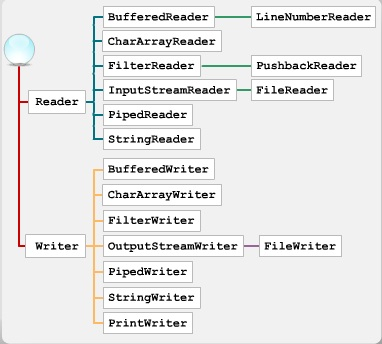
\includegraphics[]{res/img/io}
	\caption{Gerarchia Reader/Writer}
\end{figure}

In Java le operazioni di input e output sono trattate considerando i dati come flusso (stream). Lo stream é un'astrazione dei dispositivi di input/output: si apre lo stream, si leggono/scrivono i dati, si chiude lo stream.

In Java gli stream sono istanze di classi raccolte nel package \texttt{java.io}. Il pacchetto contiene due gerarchie di classi in base al tipo di flusso:
\begin{itemize}
 \item flusso di caratteri, usati per la lettura/scrittura di testo
 \item flusso di byte, usati per la trasmissione di dati in codice binario
\end{itemize}
Alla base delle gerarchie si trovano delle classi astratte con le operazioni di base:

\begin{lstlisting}
class Reader{
	int read()
	int read(char[] buff)
	abstract int read(char[] buff, int off, int cnt)
	int skip(long count)
	abstract void close()
	boolean ready()
}

class Writer{
	void write(char b)
	void write(String r)
	abstract void write(char[] buff, int off, int cnt)
	abstract void close()
	abstract void flush()
}

class InputStream{
	abstract int read()
	int read(byte[] buff)
	int read(byte[] buff, int off, inf cnf)
	int skip(long count)
	void close()
	boolean available()
}

class OutputStream{
	abstract void write(byte b)
	void write(byte[] buff)
	void write(byte[] buff, int off, int cnt)
	void close()
	void flush()
}
\end{lstlisting}
Alcuni gruppi di classi che estendono le precedenti:
\begin{itemize}
\item flussi \texttt{Filter}, che hanno un qualche filtro
\item flussi \texttt{Buffered}, che aggiungono la presenza di un buffer per ridurre gli accessi ai dispositivi di input/output
\item flussi \texttt{Piped}, che sono coppie di flussi in cui si legge in uno e si scrive nell'altro
\end{itemize}
I flussi standard (tastiera e video), sono flussi di byte.

\section{Stream e file}
Quando si trasmette con un file, serve la classe adeguata. Per i caratteri si usa \texttt{FileReader} e \texttt{FileWriter}, mentre per i byte si usa \texttt{FileInputStream} e \texttt{FileOutputStream}.
L'accesso al file può essere sequenziale o diretto.

\begin{lstlisting}
import java.io.*;
public class Demo {
public static void main(String[] a) {
  // 1. Leggere input per linee
	BufferedReader in = new BufferedReader(
		new FileReader("Demo.java")
	);
	String s, s2 = new String();
	while((s = in.readLine())!= null) s2 += s + "\n";
	in.close();

	// 2. Leggere dallo standard input
	BufferedReader stdin = new BufferedReader(
		new InputStreamReader(System.in)
	);
	System.out.print("Enter a line:");
	String linea = stdin.readLine();
	System.out.println(linea);
\end{lstlisting}

\section{Serializzazione}
I dati trasmessi in input/output a volte possono essere proprio degli oggetti. Con \texttt{ObjectInputStream e ObjectOutputStream} è possibile rappresentare flussi di oggetti. 

Non tutti gli oggetti vanno bene: solo quelli che implementano l'interfaccia \texttt{Serializable}. L'interfaccia non ha metodi e serve solo a marcare che gli oggetti possono essere trasmessi tramite stream. Viene lanciata l'eccezione \texttt{NotSerializableException} se si usa un oggetto che non implementa Serializable.

La serializzazione è il processo che trasforma un oggetto in un'opportuna sequenza di byte (\texttt{writeObject(obj)}) e viceversa (\texttt{readObject()} - deserializzazione). La deserializzazione ritorna un oggetto di tipo \texttt{Object}, quindi sta al programmatore fare un cast corretto in base al tipo adatto. 

Non tutti i tipi sono serializzabili. Tuttavia quando si serializza un oggetto, devono essere serializzati tutti i campi, soprattutto se sono riferimenti ad altri oggetti che però possono essere non serializzabili. In questi casi si può implementare la serializzazione custom:
\begin{itemize}
\item la classe deve avere il costruttore senza argomenti
\item la classe deve implementare i due metodi di lettura/scrittura
\item i campi non serializzabili vanno indicati con la keyword \texttt{transient}
\end{itemize}

\section{Espressioni Lambda}
Un'espressione Lambda in Java è un metodo senza dichiarazione esplicita con una forma \texttt{(parametri) -> \{corpo\}}.
Regole generiche:
\begin{itemize}
\item i parametri possono essere più di uno, separati da virgola, ma anche nessuno
\item le parentesi dei parametri si possono omettere se è un solo parametro
\item il tipo dei parametri può essere implicito o esplicito
\item le parentesi del corpo possono venire omesse se è un solo statement
\end{itemize}

Le espressioni Lambda vengono tradotte dal compilatore in funzioni di \textbf{interfacce funzionali}. Le interfacce funzionali contengono un singolo metodo astratto con i parametri ed il corpo dell'espressione Lambda. 

\begin{lstlisting}
public interface Consumer<T> {
	void accept(T t);
}
Consumer<Integer> c = x -> System.out.println(x);
c.accept(new Integer(1));	
\end{lstlisting}

Esistono delle interfacce già definite come:
\begin{itemize}
\item \texttt{Function} - accetta un argomento di tipo T e ritorna un tipo R
	\begin{lstlisting}
Function<String, String> m = s -> s.toUpperCase();

// composizione e applicazione di g o f: String -> float
Function<String, Integer> f = String::length;
Function<Integer, Float> g = Integer::floatValue;
Function c = g.compose(f);
c.apply("PCD")
	\end{lstlisting}
\item \texttt{Supplier} - nessun argomento e ritorna un tipo R
	\begin{lstlisting}
Supplier<String> helloStrSupplier =
	() -> new String("Hello");
String helloStr = helloStrSupplier.get();
	\end{lstlisting}
\item \texttt{Consumer}   - un solo argomento e non ritorna niente. Rispetto alle altre interfacce lavora con side-effects
	\begin{lstlisting}
Consumer<Integer> c = x -> System.out.println(x);
c.accept(new Integer(1));	
someArrayList.forEach(c);
	\end{lstlisting}
\item \texttt{Predicate} - un solo argomento e ritorna boolean 
	\begin{lstlisting}
Predicate<String> p_1 = x -> x != null;
Predicate<String> p_2 = x -> x != null || x.length() > 2;
Predicate<List<String>> p_3 = x != null && s.size() > 1;
	\end{lstlisting}
\end{itemize}

\section{Stream API}
L'interfaccia \texttt{Stream} è stata introdotta da Java 8 in supporto alle operazioni sequenziali e parallele su un flusso. Uno stream \`e un insieme di oggetti, tipicamente provenienti da una collezione, array, generatore o qualche operazione di I/O ed è caratterizzato una sequenza di passi.

Uno stream è una pipeline composta da:
\begin{itemize}
	\item Un generatore di stream (sorgente, ottiene dati da elaborare)
	\item Zero o pi\`u operazioni intermediarie dette anche \textit{lazy}. Le operazioni intermedie non sono valutate fino a quando un operazione terminale viene incontrata. Ogni operazione intermedia restituisce uno stream ed aggiunge un nuovo "ingrediente" alla ricetta (pipeline di operazioni)
	\item Una singola operazione terminale che scatena l'esecuzione detta anche \textit{eager}
\end{itemize}

Non produce side-effect e a differenza delle collezioni, che sono finite, le stream sono potenzialmente infinite. Gli elementi dello stream vengono visitati una sola volta.

\begin{lstlisting}
List<Integer> list = Stream<Integer>.of(1, 2, 3)
	.filter(x -> x.intValue() > 1)
	.collect(Collectors.toList());

long count = list.stream().filter(x -> true).count();
\end{lstlisting}

\subsection{Caratteristiche}

La sorgente di uno Stream pu\`o dichiarare alcune caratteristiche che gli operatori intermedi possono verificare e che l'operazione terminale usa per prendere decisioni sulla esecuzione. L'operazione terminale ha piena visibilit\`a, prima di cominciare a lavorare, di quali sono le caratteristiche della pipeline di esecuzione, e pu\`o quindi prendere decisioni in merito.

\begin{itemize}
	\item CONCURRENT:	Parallelizzabile
	\item DISTINCT:	Elementi distinti
	\item IMMUTABLE:	Immutabile durante il consumo
	\item NONNULL:	Elementi non nulli
	\item ORDERED:	Elementi ordinati
	\item SIZED:	Dimensione nota
	\item SORTED:	Ordinamento definito
	\item SUBSIZED:	Suddivisioni di dimensione nota
\end{itemize}

\subsection{Operazioni su Stream}

Operazioni su stream, che possono essere intermedie (ritornano un nuovo stream) o terminali (ritornano un valore):

\begin{itemize}
\item \texttt{filter()} [Intermedia] - ritorna uno stream con gli elementi filtrati secondo il predicato passato 
\item \texttt{map()} [Intermedia] - ritorna uno stream con gli elementi ai quali ho applicato la funzione passata 
\item \texttt{flatMap()} [Intermedia] - rimpiazza ogni elemento dello stream di partenza con un nuovo stream e ritorna uno stream finale con tutti gli elementi degli stream interni. Ad esempio (viene usato un array per semplificare): \texttt{[1, 2, 3] -> [[1, 1], [2, 2], [3, 3]] -> [1, 1, 2, 2, 3, 3]} 
\item \texttt{distinct()} [Intermedia] - ritorna uno steam con elementi distinti 
\item \texttt{sorted()} [Intermedia] - ritorna uno stream con gli elementi ordinati 
\item \texttt{parallel()} [Intermedia] - ritorna uno stream la cui esecuzione è parallela 
\item \texttt{sequential()} [Intermedia] - ritorna uno stream la cui esecuzione è sequenziale
\item \texttt{limit()} [Intermedia] - ritorna uno stream limitato nella lunghezza in base al valore passato 
\item \texttt{collect()} [Terminale] - riduce gli elementi ad un unico valore, che solitamente è una lista
\item \texttt{forEach()} [Terminale] - compie un azione per ogni elemento dello stream 
\item \texttt{count()} [Terminale] - ritorna il numero di elementi dello stream 
\item \texttt{anyMatch()} [Terminale] - ritorna true se un qualsiasi elemento rende true il predicato; può non valutarli tutti 
\item \texttt{allMatch/noneMatch()} [Terminale] - ritorna true se tutti/nessuno degli elementi rendono true il predicato 
\end{itemize}

Maggiori esempi ed informazioni sono presenti all'articolo \url{http://winterbe.com/posts/2014/07/31/java8-stream-tutorial-examples/}.
